\documentclass[a4paper, 12pt]{article}
\usepackage[utf8]{inputenc}
\renewcommand\familydefault{\sfdefault}
\usepackage[T1]{fontenc}
\usepackage[francais]{babel}
\usepackage[left=2.5cm,top=2.5cm,right=2.5cm,bottom=2.5cm]{geometry}
\usepackage[onehalfspacing]{setspace}
\usepackage{graphicx}
\usepackage[usenames, dvipsnames]{xcolor}
\definecolor{mygray}{gray}{0.95}

\usepackage{minted}
\usemintedstyle{colorful}
\usepackage{float}
\floatplacement{figure}{H}
\usepackage{authblk}
\usepackage{enumitem}
\setlist[enumerate]{label*=\arabic*.}
\usepackage{hyperref}
\hypersetup{
    colorlinks,
    citecolor=black,
    filecolor=black,
    linkcolor=black,
    urlcolor=blue
}

\usepackage{caption}
\newenvironment{code}{\captionsetup{type=listing}}{}
\usepackage{array}
\usepackage{etoolbox}
\patchcmd{\thebibliography}{\section*{\refname}}{}{}{}

\usepackage{dirtree}
\usepackage{tabularx}

\usepackage{glossaries}
	\let\oldnewacronym\newacronym
	\newcommand*{\provideacronym}[3]{%
	  \ifglsentryexists{#1}{%
	  }{%
	    \oldnewacronym{#1}{#2}{#3}%
	  }%
	}
\makeglossaries


\begin{document}

\title{Conception d'un système de "tagging" des fichiers avec Rust}
\author{Steven Liatti}
\affil{\small Projet de bachelor - Prof. Florent Glück}
\affil{\small Hepia ITI 3\up{ème} année}
\maketitle

\subparagraph{Résumé}
Le but de ce projet est de concevoir et développer un "moteur de gestion de tags" pouvant gérer des dizaines de milliers
de fichiers et tags associés de manière efficace, en Rust. Le stockage des tags utilisera le mécanisme des "extended
attributes" disponibles dans la plupart des systèmes de fichiers modernes. Le moteur d'indexation devra surveiller les
fichiers modifiés, créés, ou supprimés afin d'indexer les tags avec un minimum de latence (temps réel). Si le temps le
permet, le système développé sera intégré à un environnement desktop choisi (Gnome, KDE, etc.).

% \begin{figure}
% 	\begin{center}
% 		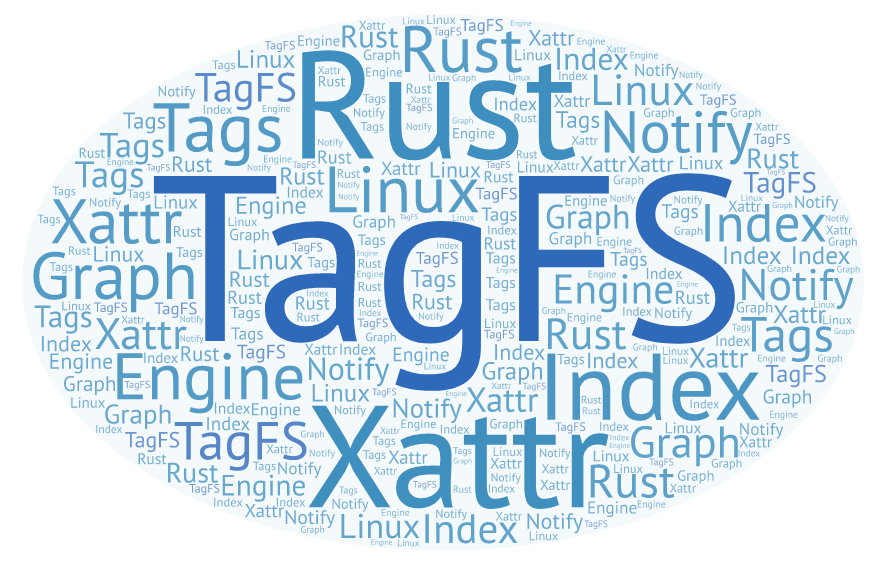
\includegraphics[width=0.43\textwidth]{images/title.png}
% 	\end{center}
% \end{figure}

\begin{figure}[!b]
	\centering
	\begin{minipage}{.4\textwidth}
		\centering
		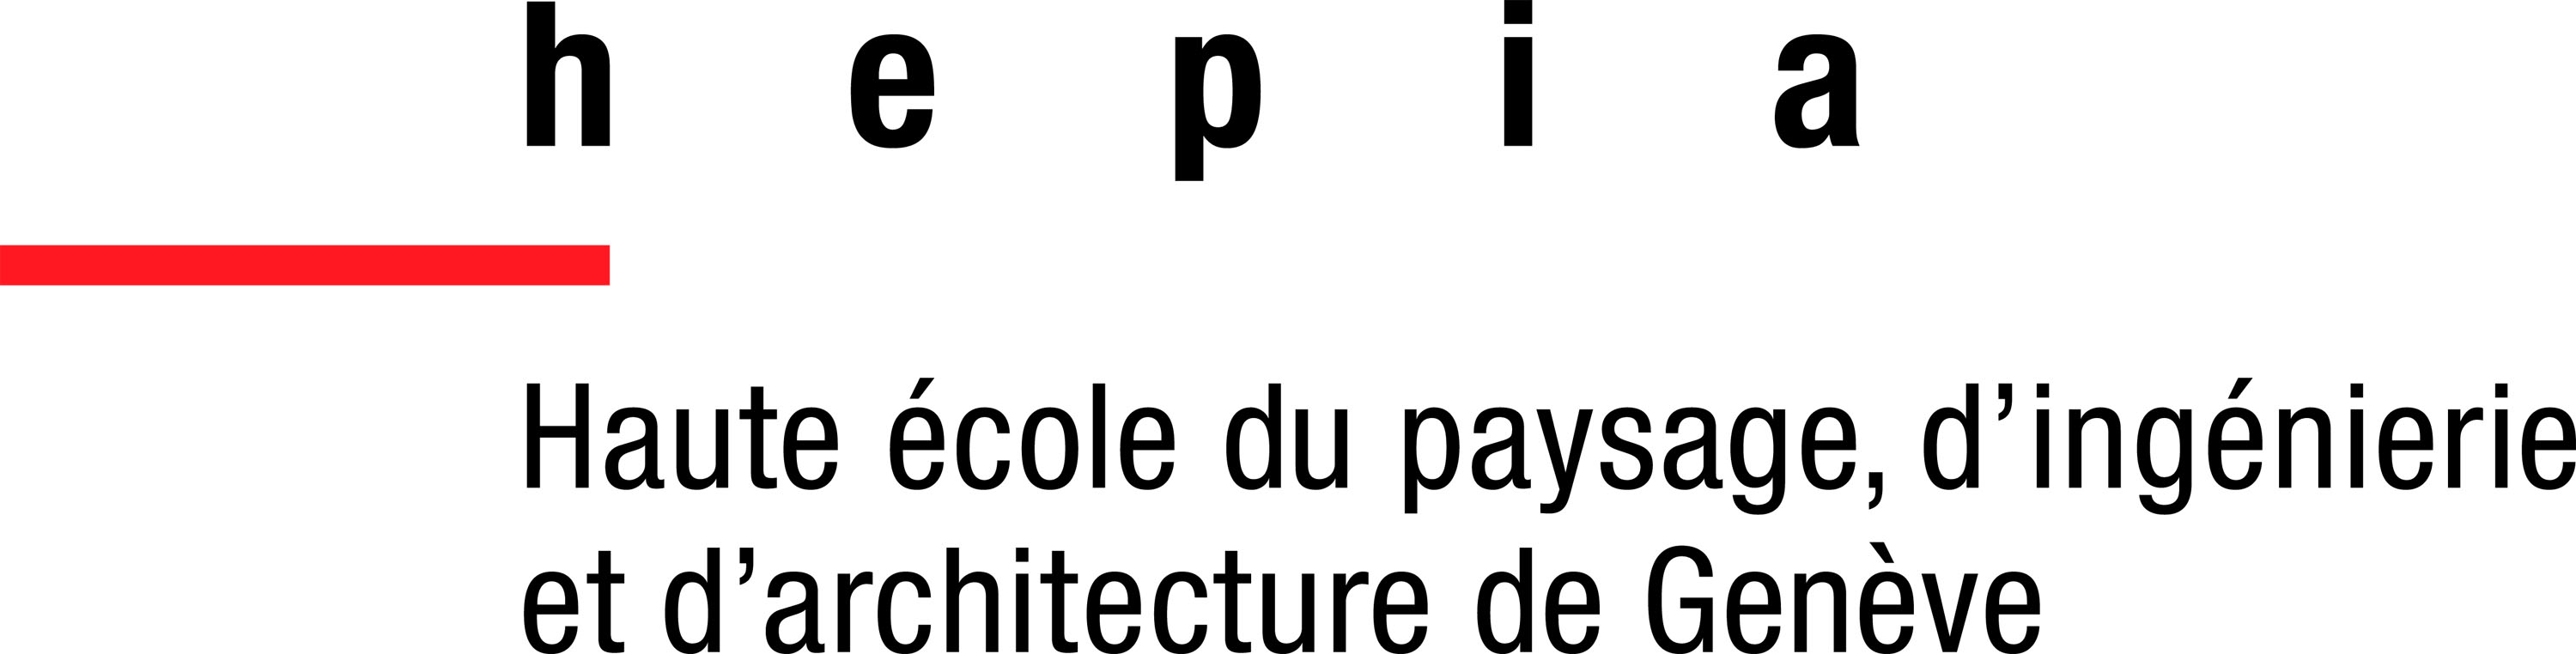
\includegraphics[width=.6\linewidth]{images/hepia.jpg}
	\end{minipage}%
	\begin{minipage}{.4\textwidth}
		\centering
		
\includegraphics[width=.6\linewidth]{images/hesso.jpg}
	\end{minipage}
\end{figure}
\newpage

\newpage

% \setcounter{tocdepth}{2}
\tableofcontents
\newpage
\listoffigures
\newpage
\listoftables
\newpage
\renewcommand\listoflistingscaption{Table des listings de code source}
\listoflistings
\newpage

\section*{Conventions typographiques} %-----------------------------------------------------------------------------------------------
Lors de la rédaction de ce document, les conventions typographique ci-dessous ont
été adoptées.
\begin{itemize}[label=\textbullet]
	\item Tous les mots empruntés à la langue anglaise ont été écrits en \textit{italique}
	\item Toute référence à un nom de fichier (ou dossier), un chemin d'accès, une 
    utilisation de paramètre, variable, commande utilisable par l'utilisateur, ou extrait de code 
    source est écrite avec une police d'écriture à \mintinline{text}{chasse fixe}.
	\item Tout extrait de fichier ou de code est écrit selon le format suivant:
    \bigbreak
    \begin{code}
        \begin{minted}[bgcolor=mygray,breaklines,breaksymbol=,linenos,frame=single,stepnumber=1,tabsize=2]{rust}
fn main() {
    println!("Hello, world!");
}
        \end{minted}
    \end{code}
\end{itemize}

\section*{Remerciements} %-----------------------------------------------------------------------------------------------
% TODO:

\newpage

% TODO: parcourir le texte pour voir si remplacement par acronyme
\newacronym{xattr}{XATTR}{\textit{Extended Attributes}, attributs étendus : voir section 
    \ref{extended_attributes}}
\newacronym{api}{API}{\textit{Application Programming Interface}, Interface de programmation : 
    services offerts par un programme producteur à d'autres programmes consommateurs}
\newacronym{syscall}{SYSCALL}{\textit{System call}, Appel système : lorsqu'un programme a besoin d'un 
    accès privilégié à certaines parties du système d'exploitation (système de fichier, mémoire, 
    périphériques), il demande au noyau d'exécuter l'opération voulue pour lui}
\newacronym{fs}{FS}{\textit{File System}, Système de fichiers : organisation logique des fichiers 
    physiques sur le disque}
\newacronym{os}{OS}{\textit{Operating System}, Système d'exploitation : couche logicielle entre le 
    matériel d'un ordinateur et les applications utilisateurs. Offre des abstractions pour la gestion 
    des processus, des fichiers et des périphériques entre autres}
\printglossary[type=\acronymtype,title={Acronymes}]
\newpage


\section{Introduction} %-----------------------------------------------------------------------------------------------
% TODO:
\acrshort{xattr}
\subsection{Motivations}
\subsection{Buts}
\cite{ref3}
% surveillance des fichiers
% indexation
% peu de latence
% temps réel
% périph amovible garde index
% rust
% efficace et peu de mémoire
% bcp de fichiers (million)
\newpage

\section{Analyse de l'existant} %-----------------------------------------------------------------------------------------------
Dans cette section, nous allons analyser les principales solutions existantes, qu'elles soient 
sous la forme d'applications utilisateur ou intégrées directement dans un \acrshort{os}.
Jean-Francois Dockes en dresse également une liste avec avantages et inconvénients sur son site 
\cite{ref3}.

\subsection{Applications utilisateur}
\subsubsection{TMSU}
TMSU \cite{ref15} est un outil en ligne de commande (CLI) qui permet d'attribuer des tags à des 
fichiers et d'exécuter des recherches par tags. On commence par initialiser TMSU dans le dossier choisi. 
Une commande liste les tags associés à un ou 
plusieurs fichiers et une autre liste les fichiers qui possèdent le ou les tags donnés. TMSU offre 
la possibilité à l'utilisateur de "monter" un \acrshort{fs} virtuel avec FUSE (Filesystem in 
UserSpacE). L'outil est rapide et efficace, mais il comporte quelques défauts :
\begin{itemize}
    \item Pas d'interface graphique
    \item Dépendance à FUSE pour monter le \acrshort{fs} virtuel
    \item Stockage des tags dans une base de données SQLite
\end{itemize}

\subsubsection{Tagsistant}
Tagsistant \cite{ref16} est autre outil CLI de gestion de tags. Il dépend de FUSE et d'une base 
de données (SQLite ou MySQL) pour fonctionner. Comme pour TMSU, il faut donner un dossier à Tagsistant 
pour son usage interne. À l'intérieur de ce dernier, se trouvent différents dossiers :
\dirtree{%
.1 /.
.2 alias --- Dossier contenant les requêtes les plus courantes.
.2 archive --- Dossier listant les fichiers.
.2 relations --- Dossier contenant les relations entre les tags et fichiers.
.2 stats --- Dossier contenant des infos sur l'utilisation de Tagsistant.
.2 store --- Dossier où sont taggés les fichiers.
.2 tags --- Dossier de gestion des tags.
}
\bigbreak
Chaque dossier a un rôle bien précis. Tout se fait avec le terminal et des commandes usuelles 
(\mintinline{text}{cp}, \mintinline{text}{ls}, \mintinline{text}{mkdir}, etc.). Dans Tagsistant, 
un dossier créé dans le dossier \mintinline{text}{tags} correspond à un tag. On se retrouve 
finalement avec une arborescence de tags et de fichiers \cite{ref17}. Bien que cet outil soit 
performant d'un point de vue de la rapidité d'exécution, il comporte les défauts de TMSU ainsi que 
des nouveaux :
\begin{itemize}
    \item Pas d'interface graphique
    \item Dépendance à FUSE pour monter le \acrshort{fs} virtuel
    \item Stockage des tags dans une base de données
    \item Utilisation des différents dossiers peu intuitive
\end{itemize} 

\subsubsection{TaggedFrog}
TaggedFrog \cite{ref18} est un programme disponible sur Windows uniquement et ne partage pas ses sources.
Son fonctionnement interne n'est pas documenté. L'interface est agréable, on peut ajouter des fichiers 
par Drag \& Drop. L'interface créé au fur et à mesure un "nuage" de tags, comme on peut le retrouver sur 
certains sites web. On peut exécuter des recherches sur les tags et les fichiers. On peut supposer que 
TaggedFrog maintient une base de données des tags associés aux fichiers, ce qui ne correspond à nouveau 
pas à nos besoins.
\begin{figure}
    \begin{center}
        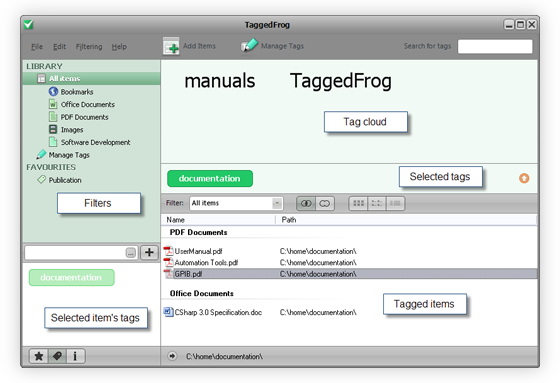
\includegraphics[width=0.8\textwidth]{images/taggedfrog.png}
    \end{center}
    \caption{TaggedFrog en utilisation \cite{ref18}}
    \label{taggedfrog}
\end{figure}

\subsubsection{TagSpaces}
TagSpaces \cite{ref13} est un programme avec une GUI permettant d'étiqueter ses fichiers avec des tags. 
L'application est agréable à utiliser, on commence par connecter un emplacement qui fera office de dossier de 
destination aux fichiers. On peut ajouter ou créer des fichiers depuis l'application. Les fichiers 
existants ajoutés depuis l'application sont copiés dans le dossier (cela créé donc un doublon). 
Sur le panneau de gauche se situe la zone de gestion des tags. TagSpaces ajoute automatiquement 
certains tags dits "intelligents" aux fichiers nouvellement créés avec l'application (par exemple 
un tag avec la date de création).
\begin{figure}
    \begin{center}
        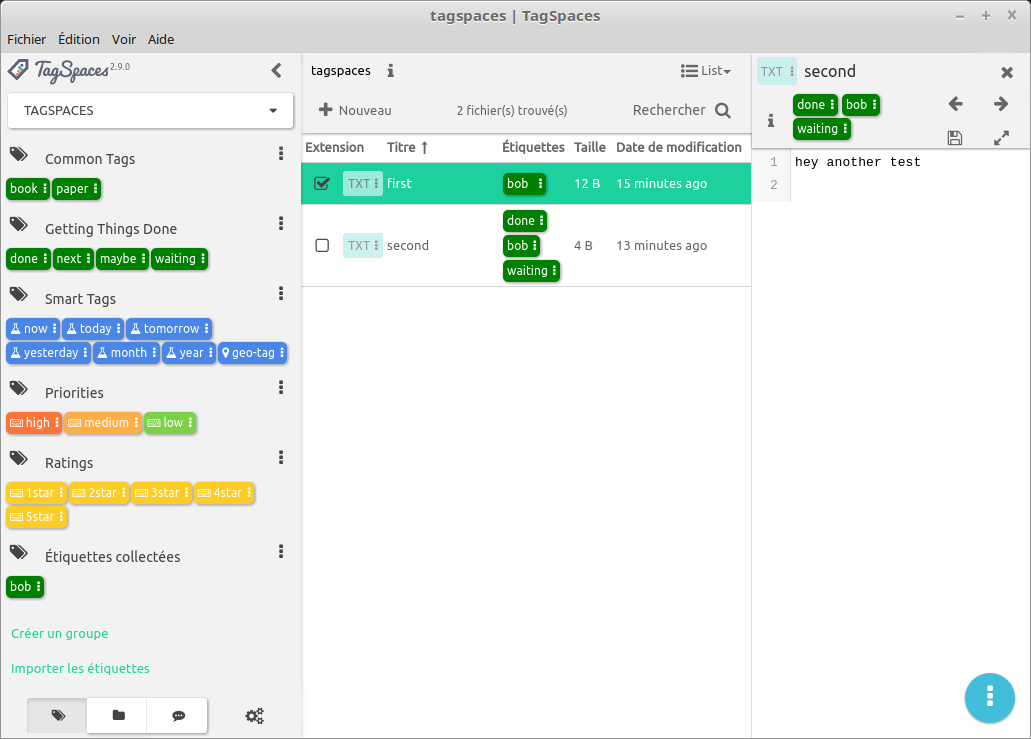
\includegraphics[width=0.8\textwidth]{images/tagspaces.png}
    \end{center}
    \caption{TagSpaces en utilisation}
    \label{tagspaces}
\end{figure}
Globalement, l'application est fonctionnelle et \textit{user friendly}. Cependant, 2 points noirs 
sont à déplorer :
\begin{enumerate}
    \item L'application copie les fichiers déjà existants sélectionnés par l'utilisateur, ce qui 
        créé une contrainte supplémentaire dans la gestion de ses fichiers personnels.
    \item TagSpaces stocke les tags directement dans le nom du fichier, modifiant ainsi son nom \cite{ref14}.
        Bien que pratique dans le cas d'une synchronisation à l'aide d'un service cloud, 
        le fichier devient dépendant de TagSpaces, si l'utilisateur décide de changer son nom sans 
        respecter la nomenclature interne, il risque de perdre les tags associés au fichier.
\end{enumerate}

\subsection{Fonctionnalités incluses dans l'\acrshort{os}}
% \subsubsection{BeOS}
% \subsubsection{Linux}

\subsubsection{Windows}
À partir de Windows Vista, Microsoft a donné la possibilité aux utilisateurs d'ajouter des 
méta-données aux fichiers; parmi ces méta-données se trouvent les tags. Il existe une fonctionnalité 
appelée \textit{Search Folder} qui permet de créer un dossier virtuel contenant le résultat d'une 
recherche sur les noms de fichiers ou d'autres critères \cite{ref19}. Depuis Windows 8, l'utilisateur 
a la possibilité d'ajouter des méta-données à certains types de fichiers (ceux de la suite office 
par exemple), dont des tags. Il peut par la suite exécuter des recherches ciblées via recherche de 
l'explorateur de fichiers Windows du type \mintinline{text}{meta:value} \cite{ref20}. C'est 
dommage que Windows ne prenne pas en compte davantage de types de fichiers, comme les PDFs ou les 
fichiers \mintinline{text}{.txt}.

\subsubsection{macOS}\label{existant_macOS}
macOS possède son propre système pour étiqueter des fichiers. Il est intégré depuis la version 
OS X 10.9 Mavericks. Depuis l'explorateur de fichiers, l'utilisateur a la possibilité 
d'ajouter, modifier, supprimer et rechercher des tags. Les fichiers peuvent avoir plusieurs tags 
associés. Un code couleur permet de plus facilement se souvenir et visualiser les tags attribués. 
Dans l'explorateur de fichiers, les tags se retrouvent sur le bas côté, pour y accéder plus 
rapidement. 
\begin{figure}
    \begin{center}
        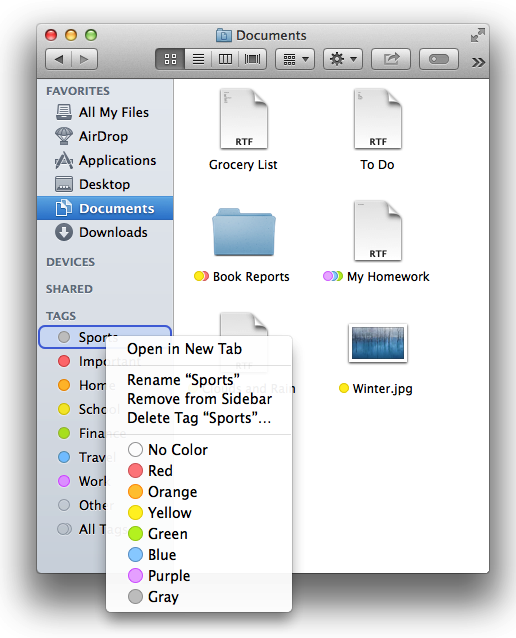
\includegraphics[width=0.8\textwidth]{images/macos_tags.png}
    \end{center}
    \caption{Vue et gestion d'un tag dans le Finder macOS \cite{ref5}}
    \label{macos_tags}
\end{figure}
Lorsque l'on clique sur un tag, une recherche Spotlight est effectuée. Spotlight est le moteur de 
recherche interne à macOS. Spotlight garde un index des tags, fournissant un accès rapide aux 
fichiers correspondants \cite{ref9}.
Tous ces tags peuvent se synchroniser sur les différents "iDevices" via iCloud. Finalement, 
un menu de réglages permet la gestion des tags (affichage, suppression, etc.) \cite{ref5}, 
\cite{ref6}. L'implémentation de ce système utilise les extended attributes (voir section 
\ref{extended_attributes}) pour stocker les tags. Les différents tags se trouvent dans l'attribut 
\mintinline{shell}{kMDItemUserTags}, listés les uns à la suite des autres. Via le Terminal, à 
l'aide de la commande \mintinline{shell}{mdls}, nous pouvons afficher la liste des tags associés à 
un fichier, nommé "Hello" pour l'exemple :
\begin{code}
    \begin{minted}[bgcolor=mygray,breaklines,breaksymbol=,linenos,frame=single,stepnumber=1,tabsize=2]{shell}
% mdls -name kMDItemUserTags Hello 
kMDItemUserTags = (
    Green,
    Red,
    Essential
)
    \end{minted}
    \caption{\mintinline{shell}{mdls} listant les tags d'un fichier sous macOS \cite{ref7}}
\end{code}
\bigbreak
Ici, ce fichier "Hello" est étiqueté avec trois tags, "Green", "Red" et "Essential". Le fait que 
l'indexation est réalisée avec Spotlight implique une réindexation des fichiers dans le cas d'un 
changement de nom pour un tag donné sous macOS. Le framework système \mintinline{text}{FSEvents} 
donne une solution partielle : c'est une \acrshort{api} (utilisée également par Spotlight) qui offre aux 
applications la possibilité d'être notifiées si un changement a eu lieu sur un dossier (un événement 
toutes les 30 secondes). \mintinline{text}{FSEvents} maintient des logs de ces changements dans 
des fichiers, les applications peuvent ainsi retrouver l'historique des changements quand elles 
le veulent \cite{ref10}.

\newpage



\section{Architecture} %-----------------------------------------------------------------------------------------------
% TODO:
% 2 index (clé -> valeur) :
% index dense, index inversé
% TODO: différence entre indexation stricte et celle réalisée ici

Le système global est composé de trois entités distinctes, décrites ci-dessous.

\subsection{Gestion des tags}
La gestion physiques des tags stockés dans les \acrshort{xattr} est une fonctionnalité indépendante du 
reste du système. Comme vu dans la section \ref{extended_attributes}, des outils système existent pour 
manipuler les \acrshort{xattr} des fichiers. Cependant, pour offrir un plus haut niveau d'abstraction, 
une cohérence sur le nommage des tags pour l'indexation et plus de confort pour l'utilisateur final, 
un outil devient nécessaire pour la gestion des tags. Cet outil se présente, sous sa forme de base, 
comme un programme en ligne de commande. Il doit, au minimum, offrir la possibilité de lire les tags 
contenus dans les fichiers et ajouter et supprimer les tags donnés en entrée par l'utilisateur. 
Il devra pouvoir manipuler plusieurs tags et fichiers simultanément. D'un point de vue algorithmique 
et structures de données, cette partie n'est pas particulièrement ardue.

\subsection{Indexation des fichiers et des tags}
L'indexation des fichiers et des tags associés est l'un des deux piliers du système. Il faut créer 
un index des relations entre les tags et les fichiers. Deux architectures ont été imaginées pour 
l'indexation des tags et des fichiers.

\subsubsection{Indexation avec table de hachage et arbre}\label{indexation_hashmap_arbre}
La première version de l'architecture de l'indexation a été la suivante, comportant deux structures 
de données :
\begin{enumerate}
    \item Une table de hachage (ou \textit{hashmap}) associant un tag (son nom, sous forme de 
        chaine de caractères) à un ensemble (au sens mathématique) de chemins de fichiers sur 
        le disque.
    \item Un arbre, correspondant à l'arborescence des fichiers, avec comme noeuds les dossiers, 
        sous-dossiers et fichiers. Le dossier à surveiller représente la racine de l'arbre.
        Les liens entre les noeuds représentent le contenu d'un répertoire. L'étiquette du noeud 
        contient le nom du fichier ou du répertoire et l'ensemble des tags associés au fichier.
\end{enumerate}
\begin{figure}
    \begin{center}
        \fbox{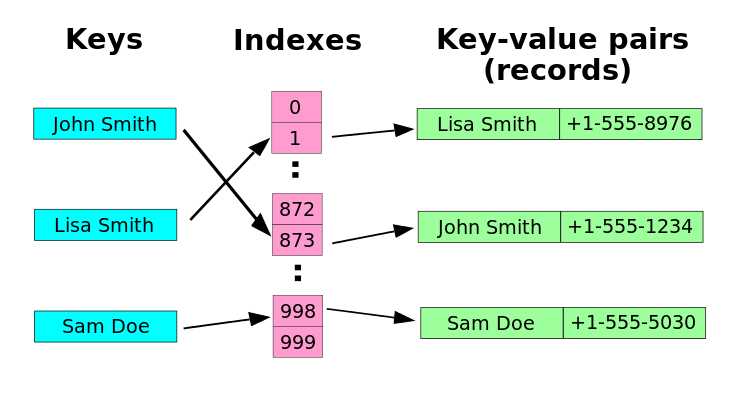
\includegraphics[width=1\textwidth]{images/hashmap_wiki.png}}
    \end{center}
    \caption{Un annuaire représenté comme une table de hachage - \cite{ref27}}
    % \label{label}
\end{figure}
Une table de hachage est un tableau associatif. Les composantes de l'association sont la "clé", 
reliée à une ou plusieurs valeurs. Pour insérer, accéder ou supprimer une entrée de la table, 
il faut calculer le "hash" de la clé, c'est-à-dire son empreinte unique. Sur l'image précédente, 
nous apercevons les clés en bleu, le résultat du hash en rouge et les valeurs associées en vert. 
Le risque que deux clés ou plus produisent une même empreinte s'appelle une "collision", c'est 
pour cela qu'une bonne implémentation d'une table de hachage doit non seulement utiliser une bonne 
fonction de hachage mais aussi une manière de résoudre les collisions. C'est ainsi que les trois 
opérations ci-dessus peuvent être réalisées, en moyenne, en temps constant (O(1)) et dans le pire 
des cas (si les collisions s'enchainent) en temps linéaire (O(n)). Dans notre cas, l'utilisation 
d'une table de hachage pour stocker la relation entre un tag et ses fichiers est efficace lorsque 
une recherche par tags est demandée. De plus, en associant un ensemble de chemins de fichiers, 
des opérations ensemblistes (union, intersection) peuvent être réalisées lorsque une recherche 
impliquant plusieurs tags est effectuée.
\bigbreak
L'arbre, au sens informatique, est une représentation de la hiérarchie du \acrshort{fs} dans 
notre cas. Prenons comme exemple la hiérarchie suivante :
\dirtree{%
.1 home.
.2 root.
.2 user.
.3 docs.
.4 graph.pdf.
.4 report.tex.
.3 images.
.4 img1.png.
.4 img2.png.
.3 music.
.4 kiss.mp3.
}
Elle peut être obtenue grâce à la commande \mintinline{bash}{tree} sous Linux par exemple.
La même représentation sous forme d'un arbre est dessinée sur l'image suivante :
\begin{figure}
    \begin{center}
        \fbox{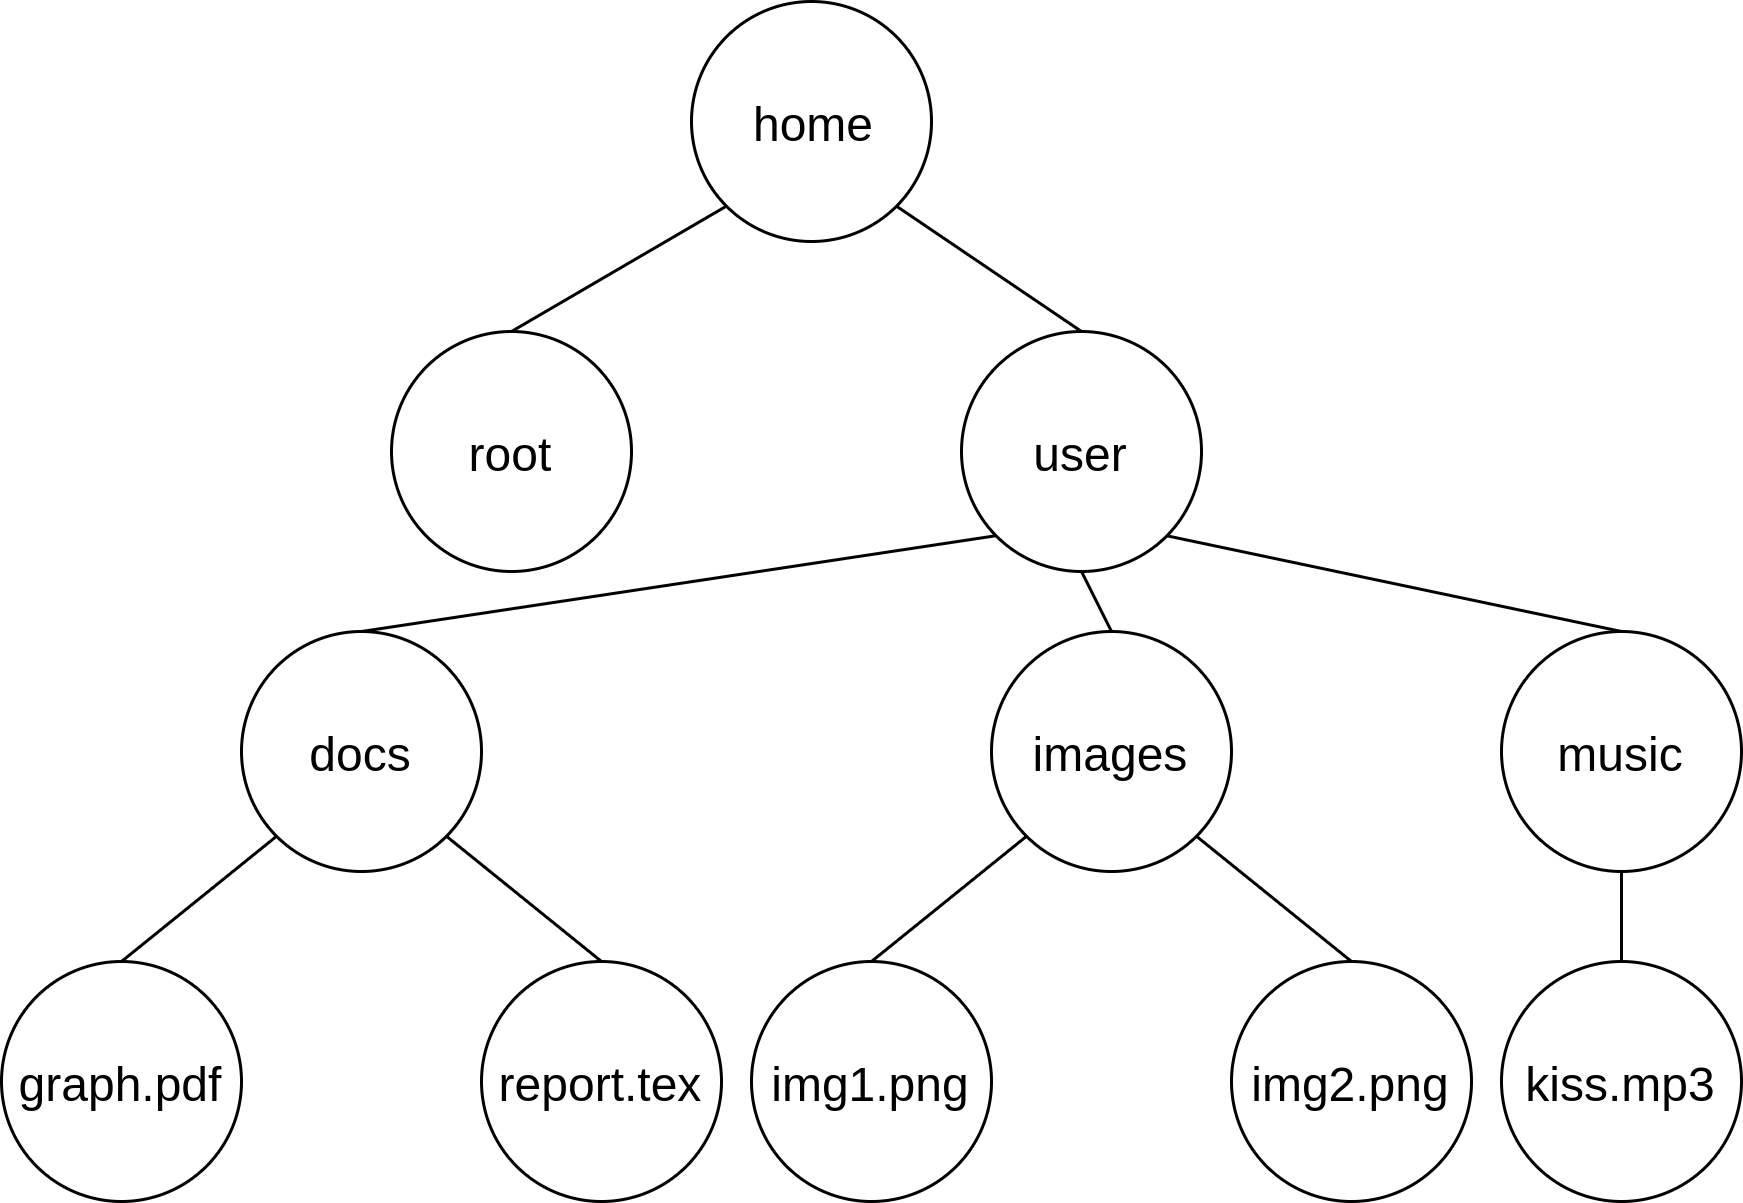
\includegraphics[width=1\textwidth]{images/tree.png}}
    \end{center}
    \caption{Représentation sous forme d'arbre d'une hiérarchie de fichiers et dossiers}
    % \label{label}
\end{figure}
Le noeud "home" représente la racine de l'arbre. Chaque noeud représente soit un fichier, soit 
un répertoire sur le disque. Chaque dossier peut être vu comme un sous-arbre de l'arbre principal.
Du point de vue programmatoire, un noeud serait définit, au minimum, comme une structure de données 
contenant un champ "données" (dans notre cas, le nom du fichier/répertoire et l'ensemble de ses tags) 
et un champ "enfants", une liste ou un ensemble de pointeurs vers les noeuds enfants. Dans le cas 
présent, seuls les noeuds répertoires pointent vers des noeuds répertoires ou fichiers enfants, 
les fichiers n'auraient qu'une liste vide de pointeurs.
\\
Le tableau \ref{tableau_architecture_1} donne un aperçu des différents cas de figure de l'utilisation du système 
de fichiers. Pour chaque cas d'utilisation, l'opération correspondante pour les deux structures de 
données (la table de hachage et l'arbre) est donnée, avec une approximation de la complexité de 
l'opération en utilisant la notation \textit{Big O}. Les variables suivantes sont définies :
\begin{itemize}
    \item $c = Operation \ constante$
    \item $p = Profondeur \ de \ l'arbre$
    \item $t = Nombre \ de \ tags$
\end{itemize}
\begin{center}
    \begin{tabularx}{16cm}{|p{3cm}|p{5cm}|X|} \hline
        \textbf{Cas d'utilisation} & \textbf{Opération \textit{hashmap}} & \textbf{Opération arbre} \\ \hline
        Ajout d'un tag à un fichier/répertoire & Si tag non présent, ajouter le tag comme clé et 
            ajouter le chemin du fichier à l'ensemble -> $O(c)$ & Parcourir l'arbre à la recherche 
            du fichier et ajouter le tag à l'ensemble des tags existants -> $O(p * c)$ \\ \hline
        Suppression d'un tag d'un fichier/répertoire & Supprimer le fichier de l'ensemble des 
            chemins de fichiers associés au tag -> $O(c)$ & Parcourir l'arbre à la recherche 
            du fichier et supprimer le tag de l'ensemble des tags existants -> $O(p * c)$ \\ \hline
        % TODO:
        % Renommage d'un tag &  &  \\ \hline
        Ajout d'un fichier & Pour tous les tags du fichier, ajouter au besoin le tag et lui 
            associer le chemin de fichier -> $O(t * c)$ & Parcourir l'arbre à 
            la recherche du répertoire parent du fichier, ajouter le nouveau noeud et l'ensemble 
            de ses tags -> $O(p * c)$ \\ \hline
        Ajout d'un répertoire & Opération identique à l'ajout d'un fichier & Parcourir l'arbre à 
            la recherche du répertoire parent, ajouter le nouveau noeud et l'ensemble 
            de ses tags, puis, récursivement, ajouter ses enfants (sous-répertoires et fichiers) 
            -> $\approx O(p^2 * c)$ \\ \hline
        Déplacement /renommage d'un fichier & Pour tous les tags du fichier, associer le nouveau 
            chemin de fichier -> $O(t * c)$ & Parcourir l'arbre à la recherche du parent et 
            changement du lien du noeud avec son parent / simple renommage du nom dans 
            l'étiquette -> $O(p * c)$ \\ \hline
        Déplacement /renommage d'un répertoire & Pour tous les tags de tous les 
            sous-répertoires et fichiers, associer le nouveau chemin de fichier -> $O(t * p * c)$ 
            & Parcourir l'arbre à la recherche du parent et changement du lien du noeud avec son 
            parent / simple renommage du nom dans l'étiquette -> $O(p * c)$ \\ \hline
        Suppression d'un fichier & Pour tous les tags du fichier, supprimer le chemin de fichier 
            -> $O(t * c)$ & Parcourir l'arbre à la recherche du parent et suppression du lien et 
            du noeud -> $O(p * c)$ \\ \hline
        Suppression d'un répertoire & Pour tous les tags de tous les sous-répertoires et fichiers, 
            supprimer le chemin de fichier -> $O(t * p * c)$ & Parcourir l'arbre à la recherche du 
            répertoire parent, supprimer le noeud, l'ensemble de ses tags, et récursivement, ses 
            enfants (sous-répertoires et fichiers) -> $\approx O(p^2 * c)$ \\ \hline
    \end{tabularx}
    \captionof{table}{Cas d'utilisation et opérations, première architecture}
    \label{tableau_architecture_1}
\end{center}

Cette version a été en partie abandonnée et adaptée pour deux raisons majeures :
\begin{enumerate}
    \item Avoir deux structures de données interdépendantes augmente la complexité des 
        opérations de mise à jour (ajout, déplacement, suppression de fichiers et tags).
    \item L'implémentation s'est avérée plus difficile que prévue, du fait de certaines 
        contraintes de Rust (voir section \ref{tag_engine_realisation}).
\end{enumerate}

\subsubsection{Indexation avec un graphe et une table de hachage}\label{graphe_architecture}
Pendant l'implémentation de cette partie du programme (voir section \ref{tag_engine_realisation}), 
une nouvelle architecture a été imaginée. Elle reprend les bases de la précédente, mais simplifie 
la structure de données. Plutôt que de maintenir deux structures différentes, cette solution 
propose une structure de données principale, secondée par une structure secondaire, optionnelle, 
mais néanmoins efficace :
\begin{enumerate}
    \item Un graphe, avec un noeud représentant soit un répertoire, soit un fichier 
        soit un tag. Chaque noeud est une structure de données comportant un nom et type et est 
        identifié de manière unique. Grâce à cet identifiant, les noeuds sont facilement accessibles.
    \item Une table de hachage, associant le nom d'un tag à son identifiant unique en tant que 
        noeud du graphe.
\end{enumerate}
Les explications suivantes sont appuyées par le cours de Jean-François Hêche, professeur à la 
heig-vd, sur les "Graphes et Réseaux". La définition d'un graphe non orienté : "Un graphe non 
orienté est une structure formée d'un ensemble V, dont les éléments sont appelés les sommets 
ou les noeuds du graphe, et d'un ensemble E, dont les éléments sont appelés les arêtes du graphe, 
et telle qu'à chaque arête est associée une paire de sommets de V appelés les extrémités de 
l'arête." (Hêche, page 1, \cite{ref28}).
\\
La définition d'un graphe orienté : "Un graphe orienté est une structure formée d'un ensemble V, dont 
les éléments sont appelés les sommets ou les noeuds du graphe, et d'un ensemble E, dont les éléments 
sont appelés les arcs du graphe, et telle qu'à chaque arc est associé un couple de sommets de 
V (c.-à-d. un élément de $V \times V$) appelés les extrémités de l'arc." (Hêche, page 3, \cite{ref28}). 
\\
Un graphe est donc un ensemble de noeuds reliés par des arêtes ou des arcs, selon si le graphe est 
orienté ou non. Dans notre cas, l'utilisation d'un graphe n'est pas si éloignée de celle d'un arbre. 
Par ailleurs, selon la théorie des graphes, "un arbre est un graphe sans cycle et connexe" (Hêche, 
page 33, \cite{ref28}). "Sans cycle" signifie qu'un parcours du graphe est possible de telle sorte 
à ce que le noeud de départ et d'arrivée soient différents. "Connexe" définit un graphe tel que 
pour chaque paire de noeuds du graphe il existe un chemin les reliant. L'utilisation d'un tel 
graphe représente fidèlement l'arborescence du \acrshort{fs} (on garde le schéma d'un arbre) 
et simplifie grandement les opérations liées. Le fait d'ajouter les tags comme noeuds du graphe 
maintient une unique structure de données cohérente et diminue le nombre d'opérations différentes 
nécessaires lors de la mise à jour du \acrshort{fs}. Le parcours de ce graphe se fait en 
fonction du chemin de fichier donné, en gardant l'identifiant unique du noeud correspondant au 
répertoire racine, le parcours se fait de la racine vers le noeud final du chemin de fichier.
\\
La table de hachage utilisée dans cette version peut être vue comme un "cache" d'accès aux noeuds 
tags. En effet, nous pourrions nous passer de cette table de hachage et lorsqu'un accès à un tag 
est demandé, rechercher dans tout le graphe le tag en question. Cependant, cette dernière opération 
devient rapidement conséquente lorsque le graphe comporte de très nombreux noeuds. De plus, elle est 
accédée bien moins souvent que dans la première version de l'architecture, car elle est mise à jour 
uniquement lors des opérations sur les tags et non plus sur celles liées seulement aux fichiers et 
répertoires (opérations potentiellement plus lourdes).
\\
Comme pour la sous-section \ref{indexation_hashmap_arbre}, le tableau 
\ref{tableau_architecture_2} donne un aperçu des opérations sur les deux structures de données 
lorsque le \acrshort{fs} est manipulé. Les variables suivantes sont définies :
% TODO: vérifier le terme "profondeur du graphe"
\begin{itemize}
    \item $c = Operation \ constante$
    \item $p = Profondeur \ du \ graphe$
    \item $t = Nombre \ de \ tags$
\end{itemize}
\begin{center}
    \begin{tabularx}{16cm}{|p{3cm}|p{7cm}|X|} \hline
        \textbf{Cas d'utilisation} & \textbf{Opération graphe} & \textbf{Opération \textit{hashmap}} \\ \hline
        Ajout d'un tag à un fichier/répertoire & Parcourir le graphe à la recherche du fichier, 
            si besoin créer le noeud tag, et relier le noeud fichier au noeud tag -> $O(p * c)$ 
            & Si non existant, ajouter le nom du tag comme clé et son identifiant dans le graphe 
            comme valeur -> $O(c)$ \\ \hline
        Suppression d'un tag d'un fichier/répertoire & Parcourir le graphe à la recherche du 
            noeud fichier et supprimer le lien entre noeud tag et fichier. Si le noeud tag 
            n'est relié à aucun autre noeud, le supprimer -> $O(p * c)$ & Si le noeud tag 
            n'est relié à aucun autre noeud, supprimer l'entrée -> $O(c)$ \\ \hline
        % TODO:
        % Renommage d'un tag &  &  \\ \hline
        Ajout d'un fichier & Parcourir le graphe à la recherche du répertoire parent, 
            ajouter le nouveau noeud. Pour les tags existants, lier le nouveau noeud, sinon créer 
            le nouveau noeud tag correspondant -> $O(p * t * c)$ & Identique à l'ajout d'un tag à 
            fichier \\ \hline
        Ajout d'un répertoire & Parcourir le graphe à la recherche du répertoire parent, 
            ajouter le nouveau noeud. Pour les tags existants, lier le nouveau noeud, sinon créer 
            le nouveau noeud tag correspondant. Répéter pour la sous-arborescence -> $\approx 
            O(p^2 * t * c)$ & Identique à l'ajout d'un tag à fichier \\ \hline
        Déplacement /renommage d'un fichier/répertoire & Parcourir le graphe à la recherche du parent et 
            changer le lien du noeud avec son parent / simple renommage du nom dans 
            l'étiquette -> $O(p * c)$ & Pas d'opération requise \\ \hline
        Suppression d'un fichier & Parcourir le graphe à la recherche du noeud fichier et supprimer les 
            liens entre noeuds tags et noeud parent -> $O(p * t * c)$ & Pour chaque tag du fichier, 
            supprimer le noeud tag s'il n'a plus de liens vers d'autres noeuds -> $O(t * c)$ \\ \hline
        Suppression d'un répertoire & Parcourir le graphe à la recherche du noeud répertoire et supprimer les 
            liens entre noeuds tags et noeud parent. Répéter pour la sous-arborescence -> $\approx 
            O(p^2 * t * c)$ & Pour chaque sous répertoire ou sous fichier, opération identique à 
            la suppression d'un fichier \\ \hline
    \end{tabularx}
    \captionof{table}{Cas d'utilisation et opérations, deuxième architecture}
    \label{tableau_architecture_2}
\end{center}
Nous pouvons constater que les opérations sur la table de hachage sont peu nombreuses et souvent 
facultatives, ce qui se traduit par un gain sur le nombre d'opérations totales.

\subsection{Surveillance du \acrshort{fs}}
La surveillance du \acrshort{fs} et des tags associés est le deuxième pilier du système. 
L'indexation initiale est nécessaire, mais il faut également surveiller en permanence 
l'arborescence des fichiers pour garder cet index à jour. Pour y parvenir, nous allons utiliser 
\mintinline{c}{inotify} (voir section \ref{inotify_techno}), en surveillant tout particulièrement les événements 
suivants :
\begin{itemize}
    \item IN\_ATTRIB : changement sur les tags (ajout, suppression, renommage)
    \item IN\_CREATE : création de fichier/répertoire dans le répertoire surveillé. Ajouter une nouvelle surveillance si répertoire.
    \item IN\_DELETE : suppression d'un fichier/répertoire dans le répertoire surveillé
    \item IN\_DELETE\_SELF : suppression du répertoire surveillé
    \item IN\_MOVE\_SELF : suppression d'un fichier/répertoire dans le répertoire surveillé
    \item IN\_MOVE\_FROM : déplacement/renommage du répertoire (ancien nom)
    \item IN\_MOVE\_TO : déplacement/renommage du répertoire (nouveau nom)
\end{itemize}
Un thread va s'occuper d'écouter les événements du \acrshort{fs} et les inscrire dans un buffer 
tandis qu'un autre va mettre à jour le graphe pour répercuter les changements survenus en lisant 
dans ce même buffer (simple pattern producteur-consommateur).

\subsection{Recherche par tags}
% TODO:
% communication sockets
% simple programme qui attend des arguments en ligne de commande
% opérateurs logiques (OU et AND)
% liste des chemins de fichiers
% génération de symlinks ?

\newpage

\section{Technologies} %-----------------------------------------------------------------------------------------------
\subsection{Rust}
% TODO:
\cite{ref0} \cite{ref1} \cite{ref2}

\subsection{Les extended attributes}\label{extended_attributes}
\subsubsection{Théorie}
Les extended attributes, ou "attributs étendus" en français, sont un moyen d'attacher des 
méta-données aux fichiers et dossiers sous forme de paires \mintinline{text}{espace:nom:valeur}. 
L'espace de nom, ou \textit{namespace} en anglais, définit les différentes classes d'attributs. 
Dans le cadre de ce projet, l'accent est mis sur ext4 sous Linux, il actuellement 4 espaces de noms 
ou classes : \mintinline{text}{user}, \mintinline{text}{trusted}, \mintinline{text}{security} et 
\mintinline{text}{system}. L'espace qui nous intéresse est \mintinline{text}{user}. C'est là que 
l'utilisateur ou l'application, pour autant qu'il ait les droits usuels UNIX sur les fichiers, peut 
manipuler les extended attributes. Les 3 autres espaces de noms sont utilisés entre autres pour 
les listes d'accès ACL (\mintinline{text}{system}), les modules de sécurité du kernel 
(\mintinline{text}{security}) ou par \mintinline{text}{root} (\mintinline{text}{trusted})
\cite{ref11} \cite{ref12}.
Le nom est une chaine de caractères et la valeur peut être une chaine de caractères ou des données binaires. 
Les extended attributes sont stockés dans les fichiers. De nombreux \acrshort{fs} gèrent leur 
usage : ext2-3-4, XFS, Btrfs, UFS1-2, NTFS, HFS+, ZFS. Ces \acrshort{fs} sont utilisés par 
les 4 \acrshort{os} les plus répandus : Windows, macOS, Linux et FreeBSD. Windows utilise 
les extended attributes notamment dans sa gestion des permissions Unix dans le shell Linux intégré 
à Windows 10 \cite{ref21}. macOS, comme vu à la section \ref{existant_macOS}, les utilise entre 
autres dans son système de gestion des tags. La commande \mintinline{text}{xattr} permet de les 
manipuler. Sous Linux, il en existe 3 : \mintinline{text}{attr}, \mintinline{text}{getfattr} et 
\mintinline{text}{setfattr}. Sous Linux avec ext2-3-4, chaque attribut dispose d'un bloc de données 
(1024, 2048 ou 4096 bytes) \cite{ref12}.
Apple et freedesktop.org préconisent la notation DNS inversée pour 
nommer les attributs \cite{ref8}, \cite{ref24} car n'importe quel processus peut modifier les 
attributs dans l'espace utilisateur. En préfixant du nom du programme le nom de l'attribut, par 
exemple \mintinline{text}{user.myprogram.myattribute}, on diminue le risque qu'une autre 
application utilise le même nom d'attribut. Malheureusement, la plupart des outils CLI Linux 
pour manipuler les fichiers comme \mintinline{text}{cp}, \mintinline{text}{tar}, etc. ne prennent 
pas en compte les attributs avec leur syntaxe par défaut \cite{ref4}.

\subsubsection{Petites manipulations}

% TODO:
% mv préserve les xattr !
% la copie dans l'explorateur de fichiers aussi (nemo)

Pour vérifier la portabilité des extended attributes, quelques tests ont été réalisés entre un 
SSD faisant office de disque système à Linux Mint avec 2 clés USB (de 8 et 64 Go) et un emplacement 
réseau monté en NFS. Le listing suivant montre la sortie de la commande \mintinline{bash}{df}, qui 
renvoie l'utilisation des différents emplacements de stockage, dans l'ordre : le disque système, en 
ext4, la clé de 8 Go formatée une fois en FAT32, puis une autre fois en NTFS, la clé de 64 Go formatée 
en ext4 et finalement une machine virtuelle sous Debian 9 montée en NFS.
\bigbreak
\begin{code}
    \begin{minted}[bgcolor=mygray,breaklines,breaksymbol=,linenos,frame=single,stepnumber=1,tabsize=2]{text}
Sys. de fichiers        Type   Taille Utilisé Dispo Uti% Monté sur
/dev/sda2               ext4     451G    334G   96G  78% /
/dev/sdg1               vfat     7.7G    4.0K  7.7G   1% /media/pc/cle1
/dev/sdg1               fuseblk  7.7G     41M  7.7G   1% /media/pc/cle1
/dev/sdg1               ext4      59G     33G   23G  59% /media/pc/cle2
192.168.1.21:/home/user nfs4     916G    198G  673G  23% /mnt/debian
    \end{minted}
    \caption{Output de \mintinline{bash}{df -Th} : le disque système, les clés USB et le NFS}
\end{code}
\bigbreak
La démarche est la suivante : un extended attribute dans l'espace \mintinline{text}{user} avec 
comme nom \mintinline{text}{author} et comme valeur \mintinline{text}{steven} est ajouté au fichier 
\mintinline{text}{file.txt} avec \mintinline{bash}{attr}. Ce fichier est copié avec 
\mintinline{bash}{cp} en prenant garde à préserver l'attribut (option 
\mintinline{bash}{--preserve=xattr}). Une fois copié, on tente de lire le même attribut, toujours 
avec \mintinline{bash}{attr}. Les résultats sont les suivants :
\bigbreak
\begin{code}
    \inputminted[bgcolor=mygray,breaklines,breaksymbol=,linenos,frame=single,stepnumber=1,
        tabsize=2,firstline=45,lastline=49]{text}{text/test_attr.txt}
    \caption{Copie sur clé USB 8 Go, FAT32}
\end{code}
\bigbreak
\begin{code}
    \inputminted[bgcolor=mygray,breaklines,breaksymbol=,linenos,frame=single,stepnumber=1,
        tabsize=2,firstline=54,lastline=61]{text}{text/test_attr.txt}
    \caption{Copie sur clé USB 8 Go, NTFS}
\end{code}
\bigbreak
\begin{code}
    \inputminted[bgcolor=mygray,breaklines,breaksymbol=,linenos,frame=single,stepnumber=1,
        tabsize=2,firstline=66,lastline=73]{text}{text/test_attr.txt}
    \caption{Copie sur clé USB 64 Go, ext4}
\end{code}
\bigbreak
\begin{code}
    \inputminted[bgcolor=mygray,breaklines,breaksymbol=,linenos,frame=single,stepnumber=1,
        tabsize=2,firstline=78,lastline=79]{text}{text/test_attr.txt}
    \caption{Copie sur l'emplacement réseau distant, NFS}
\end{code}
\bigbreak
On constate que l'opération est infructueuse sur la clé en FAT32 et sur l'emplacement réseau monté 
en NFS alors qu'elle réussit sur les clés USB en NTFS et ext4.

\subsection{\mintinline{c}{inotify}}\label{inotify_techno}
Sous Linux, un outil (inclu au noyau) dédié à la surveillance du \acrshort{fs} existe, \mintinline{c}{inotify} 
\cite{ref29}. Comme son nom l'indique, \mintinline{c}{inotify} donne la possibilité à une application d'être 
notifiée sur des événements au niveau du système de fichiers. Une \acrshort{api} en C existe et 
offre les \acrshort{syscall} suivants :
\begin{enumerate}
    \item \mintinline{c}{int inotify_init(void)} : initialise une instance \mintinline{c}{inotify} et retourne un 
        descripteur de fichier.
    \item \mintinline{c}{int inotify_add_watch(int fd, const char *pathname, uint32_t mask)} : 
        cette fonction attend le descripteur de fichier renvoyé par \mintinline{c}{inotify_init}, 
        un chemin de fichier ou répertoire à surveiller et un masque binaire constitué des 
        événements à surveiller (voir plus loin). Il retourne un nouveau descripteur de fichier 
        qui pourra être lu avec le \acrshort{syscall} \mintinline{c}{read()}.
    \item \mintinline{c}{int inotify_rm_watch(int fd, int wd)} : appel inverse du précédent, 
        supprime la surveillance du descripteur de fichier \mintinline{c}{wd} de l'instance \mintinline{c}{inotify} 
        retournée par \mintinline{c}{fd}.
\end{enumerate}
\mintinline{c}{inotify} s'utilise comme suit : il faut initialiser l'instance (1), ajouter les fichiers et répertoires 
pour la surveillance avec le masque des événements voulus (2) et, généralement, dans une boucle, 
appeler le \acrshort{syscall} \mintinline{c}{read()} avec comme argument le descripteur de fichier 
renvoyé par \mintinline{c}{inotify_init()}. Chaque appel abouti à \mintinline{c}{read()} retourne 
la structure suivante :
\bigbreak
\begin{code}
    \begin{minted}[bgcolor=mygray,breaklines,breaksymbol=,linenos,frame=single,stepnumber=1,tabsize=2]{c}
struct inotify_event {
    int      wd;       /* Descripteur de surveillance */
    uint32_t mask;     /* Masque d'événements */
    uint32_t cookie;   /* Cookie unique d'association des
                          événements (pour rename(2)) */
    uint32_t len;      /* Taille du champ name */
    char     name[];   /* Nom optionnel terminé par un nul */
};
    \end{minted}
    \caption{Structure \mintinline{c}{inotify_event} - \cite{ref29}}
\end{code}
\bigbreak
Le champ \mintinline{c}{mask} peut prendre les valeurs suivantes (multiples valeurs autorisées, 
séparées par des "ou" logiques -> "|") :
\begin{itemize}
    \item IN\_ACCESS : accès au fichier
    \item IN\_ATTRIB : changement sur les attributs du fichier
    \item IN\_CLOSE\_WRITE : fichier ouvert en écriture fermé
    \item IN\_CLOSE\_NOWRITE : fichier ouvert en écriture fermé
    \item IN\_CREATE : création de fichier/répertoire
    \item IN\_DELETE : suppression d'un fichier/répertoire
    \item IN\_DELETE\_SELF : suppression du répertoire surveillé lui-même
    \item IN\_MODIFY : modification d'un fichier/répertoire
    \item IN\_MOVE\_SELF : suppression d'un fichier/répertoire
    \item IN\_MOVE\_FROM : déplacement/renommage du répertoire (ancien nom)
    \item IN\_MOVE\_TO : déplacement/renommage du répertoire (nouveau nom)
    \item IN\_OPEN : ouverture d'un fichier
    \item IN\_ALL\_EVENTS : macro combinant tous les événements précédents
\end{itemize}
Le champ \mintinline{c}{cookie} de la structure \mintinline{c}{inotify_event} prend tout son sens 
lors des événements IN\_MOVE : un numéro unique est généré pour faire le lien entre ces deux 
sous-événements, qui ne sont en réalité qu'un seul. \mintinline{c}{inotify} offre donc une très bonne base pour 
la surveillance du \acrshort{fs}. Il possède cependant quelques limitations :
\begin{itemize}
    \item Pas de surveillance récursive d'un répertoire : si une arborescence complète doit être 
        surveillée, il faut pour chaque sous-répertoire ajouter une surveillance dédiée.
    \item Les chemins de fichiers peuvent changer entre l'émission d'un événement et son traitement
    \item \mintinline{c}{inotify} ne permet que la surveillance de répertoires en espace utilisateur par défaut
    \item Il n'y pas de moyen de discriminer quel processus ou utilisateur a généré un événement
\end{itemize}
Il existe plusieurs outils système qui utilisent \mintinline{c}{inotify} \cite{ref30} :
\begin{itemize}
    \item \mintinline{bash}{incron} : équivalent de \mintinline{bash}{cron}, mais l'exécution 
        des tâches se fait non pas selon un horaire donné, mais selon un événement donné sur un fichier
    \item \mintinline{bash}{lsyncd} : outil de synchronisation, basé sur \mintinline{bash}{rsync}. 
        La synchronisation est effectuée à chaque changement dans le répertoire surveillé vers une 
        liste d'emplacements distants configurés à l'avance.
    \item \mintinline{bash}{iwatch} : déclenchement d'une commande selon un événement \mintinline{bash}{inotify}
    \item \mintinline{bash}{inotify-tools} : deux commandes permettant d'utiliser \mintinline{bash}{inotify} 
        directement dans le terminal :
        \begin{itemize}
            \item \mintinline{bash}{inotifywait} : exécute une attente sur un événement, avant de 
                continuer le fil d'exécution
            \item \mintinline{bash}{inotifywatch} : retourne une liste d'événements des répertoires surveillés
        \end{itemize}
\end{itemize}
Pour plus d'informations, la page de \mintinline{text}{man} sur \mintinline{c}{inotify} existe \cite{ref29} et 
un très bon article en deux parties sur les ajouts de \mintinline{c}{inotify} par rapport à \mintinline{c}{dnotify} 
(son prédécesseur) et sur ses limitations par Michael Kerrisk \cite{ref31} \cite{ref32}.
\newpage


\section{Réalisation} %-----------------------------------------------------------------------------------------------
\subsection{Tag Manager}
La première réalisation de ce projet est un outil en ligne de commande, écrit en Rust, permettant 
de facilement lister, ajouter et supprimer des tags à des fichiers et dossiers. Il fait usage de 
deux \textit{crates} disponibles sur \href{https://crates.io}{crates.io} : clap \cite{ref22} et 
xattr \cite{ref23}. Clap (Command Line Argument Parser for Rust) est une librairie pour parser 
les arguments d'un programme en ligne de commande. Xattr est une \acrshort{api} en Rust pour récupérer, lister, 
ajouter/modifier et supprimer des \acrshort{xattr} avec Rust. Elle utilise les \acrshort{syscall} 
en C fournis par Linux.
% TODO:
% Insérer quelques bouts de code intéressants. -> examples/01a_quick_example.rs pour clap
% Insérer capture/exemple d'utilisation
% Option récursive

\subsection{Tag Engine}\label{tag_engine_realisation}
\cite{ref26}
% TODO:
% Taille des index de petgraph, 32 bits = ~ 4 millions de fichiers, 64 bits = 10 puissance 19 = ~ 2 puissance 190 fichiers
% \mintinline{c}{inotify} limitations, inotifywait, dossier /media -> clé USB
\newpage

\section{Tests du système} %-----------------------------------------------------------------------------------------------
\newpage

\section{Discussion/résultats} %-----------------------------------------------------------------------------------------------
% cahier des charges rempli ?
% réalisation OK ?
% performances
% Rust VS C
% Bugs
% Améliorations futures

\newpage

\section{Conclusion} %-----------------------------------------------------------------------------------------------


\newpage
\section{Références} %-----------------------------------------------------------------------------------------------
\bibliographystyle{unsrt}
\bibliography{bib}

\end{document}

% \begin{figure}
%     \begin{center}
%         \includegraphics[width=0.8\textwidth]{images/image.png}
%     \end{center}
%     \caption{légende}
%     \label{label}
% \end{figure}

% \begin{code}
%     \begin{minted}[bgcolor=mygray,breaklines,breaksymbol=,linenos,frame=single,stepnumber=1,tabsize=2]{rust}
% fn main() {
%     println!("Hello, world!");
% }
%     \end{minted}
%     \caption{Hello world en Rust}
% \end{code}
% \bigbreak

% \begin{code}
%     \inputminted[bgcolor=mygray,breaklines,breaksymbol=,linenos,frame=single,stepnumber=1,
%         tabsize=2,firstline=157,lastline=185]{rust}{file.rs}
%     \caption{légende}
% \end{code}
% \bigbreak
